\section{Neural Networks}
\subsection{The Perceptron}
The basis of each artificial neural network is the \textit{perceptron}. A perceptron essentially is an algorithm that is inspired by biological neurons. The perceptron can therefore be understood as an artificial neuron.

Mathematically, a perceptron processes an input vector $\vec{x}\in\mathbb{R}^n$ and produces an output vector $\vec{y}\in\mathbb{R}^m$. 
%
\begin{figure} \label{fig:2.1}
    \centering
    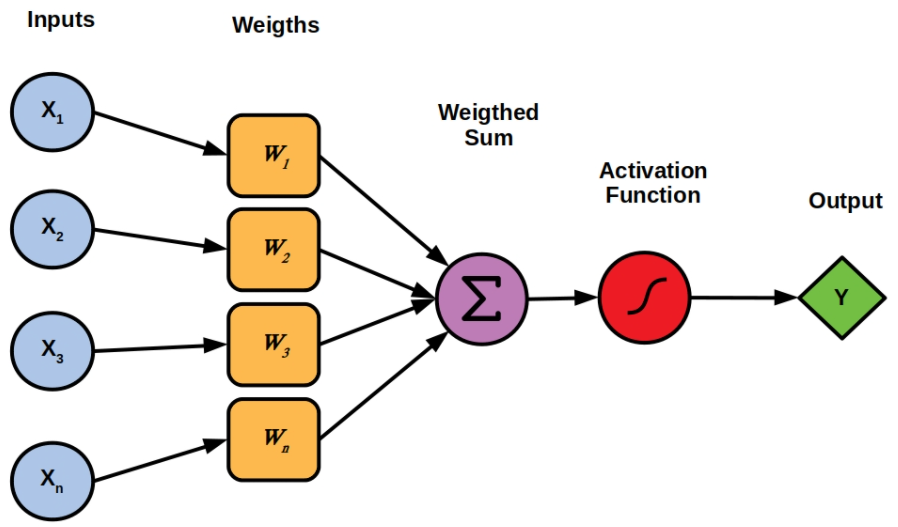
\includegraphics[width=.5\textwidth]{Chapters/figures/perceptron.PNG}
    \caption[Schematic layout of a perceptron]{Schematic layout of a perceptron. Figure from\\ https://starship-knowledge.com/neural-networks-perceptrons.}
\end{figure}
%
In the simplified representation of a perceptron in \hyperref[fig:2.1]{Fig.\,2.1} the inputs $x_i$ $ (i=0,\dots,n)$ are multiplied by weights $w_i$ and then summed. Thereafter a non-linear function is applied to produce the output $y\in\mathbb{R}$. It is the adaption of these weights to a specific problem that is the core of learning in a neural network. A generalization of the transformation described above is given by
%
\begin{equation} \label{equ:2.1}
    \vec{A}\cdot\vec{x}+\vec{b}=\vec{\hat{\vec{y}}}
\end{equation}
%
where $A\in\mathbb{R}^{m\times n}$ is a matrix of weights and $b\in\mathbb{R}^m$ is a bias. Then a non-linear transformation of the form
%
\begin{equation} \label{equ:2.2}
    \vec{y}=\varphi(\hat{\vec{y}})
\end{equation}
%
is applied to the intermediate result $\hat{\vec{y}}$. The non-linear function $\varphi(\cdot)$ is called the \textit{activation function}. This function has the task of mapping the arbitrary output $\hat{\vec{y}}$ from the range $(-\infty,\infty)$ to a more appropriate range. The choice of the activation function depends heavily on the specific architecture of a neural network. Typical choices of activation functions are the Sigmoid, Tanh, Softmax and ReLU functions. As activation functions do not play a big role in this thesis the concrete definition of these functions is left as an exploration to the reader.
%
\subsection{Multilayer Perceptrons} \label{sec:2.1.2}
A \textit{Multilayer Perceptron} is an arrangement of perceptrons in different consecutively interconnected layers. This is what we call a (very basic) \textit{Neural Network}. As depicted in \hyperref[fig:2.2]{Fig.\,2.2} a Multilayer Perceptron is composed of an input layer, one or more hidden layers and an output layer. 
%
\begin{figure} \label{fig:2.2}
    \centering
    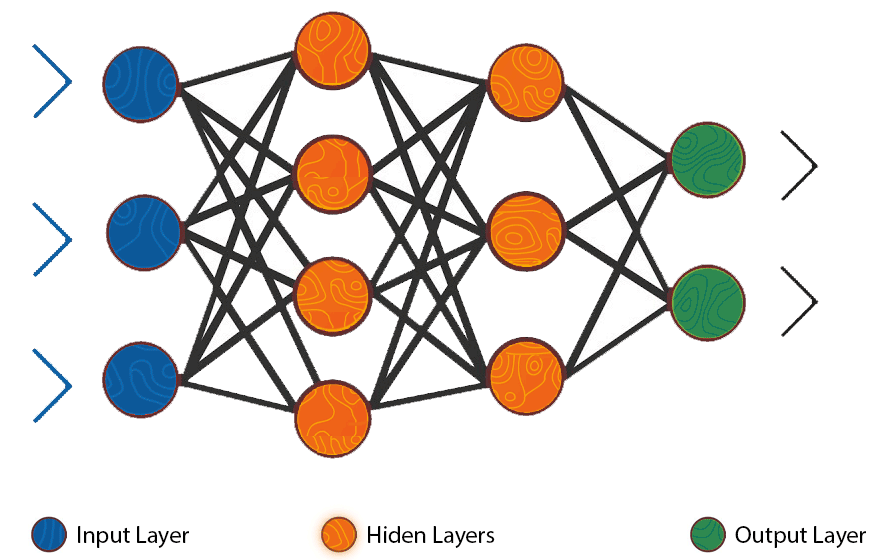
\includegraphics[width=.5\textwidth]{Chapters/figures/multilayer_perceptron.PNG}
    \caption[The Multilayer Perceptron]{The Multilayer Perceptron. Figure from\\ https://cdn.analyticsvidhya.com/wp-content/uploads/2020/02/ANN-Graph.gif}
\end{figure}
%
The output of a layer is connected to the input of the next layer (here: fully connected). The hidden layers can perform various tasks and some of them are presented in \hyperref[sec:2.1.3]{Sec.\,2.1.3}.

During training the learning process of such a neural network consists of three parts which are computed iteratively: the \textit{forward pass}, the \textit{loss calculation} and the \textit{backward pass}. In the forward pass, the input values get processed by the different layers of the neural networks to then produce an output. The loss calculation then computes how good this output is in relation to some optimal output for the given input. This is the concept of \textit{supervised learning}. There is a variety of so-called \textit{loss functions} for the calculation of losses, some of them will be discussed later in this thesis. The computed loss is then back-propagated through the network to update the parameters of each perceptron in each layer. This is the process of artificial learning. Back-propagation often works in the sense of a gradient descent. Since the loss is to be minimized, the influence of all individual parameters on the loss is then derived and adjusted according to the resulting gradient. 

Usually a batch of data is processed simultaneously by the network. While processing the whole dataset at once would lead to faster converging and overall better results in optimization with gradient decent, a larger batch size comes with a much higher vRAM cost during training. Therefore one often decides to use a mini-batch of data which makes the best possible use of the memory of the graphics card. The process of forward pass, loss computation and backward pass of one batch is then called an \textit{iteration} or a \textit{step}. After each batch has been processed in a dataset, an \textit{epoch} has passed.
%
\subsection{Common Layers in Neural Networks} \label{sec:2.1.3}
Depending on the task of the neural network, different layers of perceptrons are used. The most common ones are \textit{Fully Connected Layers}, \textit{Normalization Layers}, \textit{Convolutional Layers}, \textit{Pooling 
Layers} and \textit{Dropout \cancel{Layers}}. It is important to note that the choice of layers for a specific problem is \textbf{not} trivial! In fact, often it is not even clear why a specific layer is good for a specific task. Furthermore, when training a neural network, it is – in general – impossible to have any insight on how the neural network learned the task.
%
\subsubsection{Fully Connected Layers}
A fully connected layer is the easiest layer for neural networks. In this layer, the output of every perceptron in one layer is connected to the input of every perceptron in the next layer. Mathematically, this describes a linear operation between the perceptrons of two layers. Although fully connected layers are in theory able to fit every problem quite well (see Universal Approximation Theorem, e.g. \cite{universal_appr_theorem}) ,they cannot be used excessively. Considering a $128\times128$ pixel RGB image leads to $4,831,838,208$ parameters to learn for two fully connected layers. Learning such a high number of parameters (weights) is computationally very expensive and often not feasible.
%
\subsubsection{Normalization Layers}
Normalization layers normalize the given inputs. There are several normalization techniques that depend on the choice of what to normalize. Take Batch Normalization (BN) \cite{batch_norm} as an example. Suppose the image data is of the form $(N, C, W, H)$ where $N$ is the batch size, $C$ is the channel number (e.g. $3$ for RGB images) and $W$ and $H$ are width and height respectively. Then BN normalizes $(N, W, H)$ for each $C$ by transforming the input $\vec{x}$ in the following way:
%
\begin{equation} \label{equ:2.3}
    \mu_B=\frac{1}{N}\sum_{i=1}^Nx_i, \quad\sigma_B^2=\frac{1}{N}\sum_{i=1}^N(x_i-\mu_B)^2\quad \Longrightarrow\quad y_i=\gamma\frac{x_i-\mu_B}{\sigma_B}+\beta,
\end{equation}
%
where $\gamma$ and $\beta$ are learnable parameters of the layer. Depending on the dimensions of the input that get normalized there is also \textit{Channel Norm}, \textit{Instance Norm} and \textit{Group Norm}. Normalization layers are used to improve the stability, speed and performance of neural networks.
%
\subsubsection{Convolutional Layers}
The Convolution Layer might be the most important layer in computer vision and gives rise to the category of \textit{Convolutional Neural Networks} (CNNs) \cite{cnn}. This type of neural networks makes extensive use of convolutional layers and is an important concept in computer vision tasks as it is very good at capturing image details \cite{deep_image_prior}.

A Convolutional Layer is especially useful to extract features from images. For example, these features could be lines in different direction but as mentioned above, normally we do not know what information (features) a neural network learns in a (convolutional) layer. In general, one can only say that in a CNN of subsequent Convolutional Layers the upper layers learn more simple features such as lines and the deeper layers learn more complex features, e.g. how a car looks like. This characteristic is called \textit{receptive field} and is due to the fact that a pixel of the first convolutional layer contains information only from, for example, $9$ pixels of the image for a $3\times3$ convolution, while a deeper convolutional layer contains information from many more pixels of the image.

As the Convolutional Layer is most often used for image feature extraction, the \textit{2D-Convolution Layer} is the most popular Convolution Layer and is defined by a 2-dimensional convolution
%
\begin{equation}
    y_{i,j}=(\vec{x}\ast\vec{f})_{i,j}=\sum_{c=1}^{C}\sum_{h=1}^{H_f}\sum_{w=1}^{W_f}\vec{f}_{c,h,w}\vec{x}_{i+h-1,j+w-1,c}
\end{equation}
%
for an input of size $(C,H,W)$. Essentially this operation can be understood as applying a filter $\vec{f}$ of size $(C, H_f, W_f)$ to each part of the image. For each position of the filter the corresponding values in the image are multiplied with the learned weights in the filter and then summed up. These summed values for each filter position then form a new output. An illustration of this process is shown in \hyperref[fig:2.3]{Fig.\,2.3}.
%
\begin{figure} \label{fig:2.3}
    \centering
    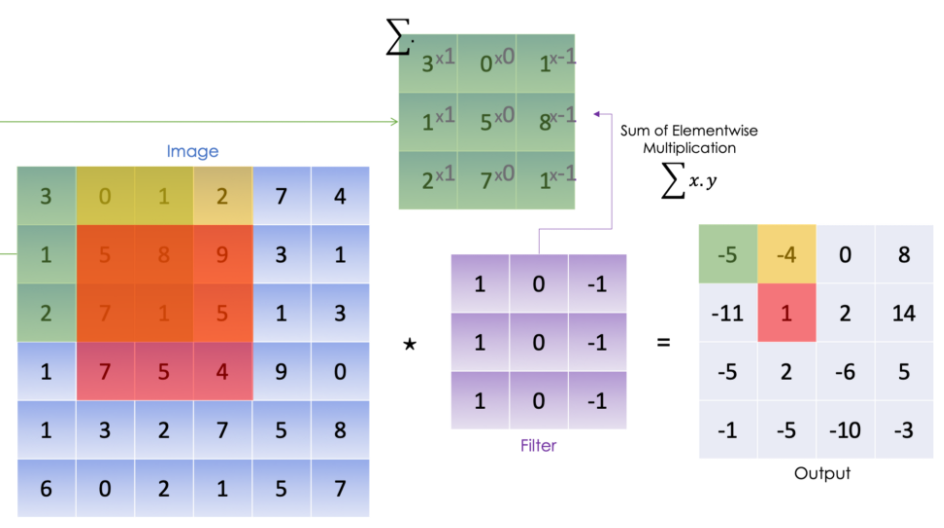
\includegraphics[width=.65\textwidth]{Chapters/figures/convolution.PNG}
    \caption[Operation principle of Convolutional Layers]{Operation principle of Convolutional Layers. Figure from\\ https://towardsdatascience.com/convolutional-neural-networks-mathematics-1beb3e6447c0.}
\end{figure}
%
\subsubsection{Pooling Layers}
As we have seen, Convolutional Layers summarize and learn specific features in an input image. These feature maps are very sensitive to the location of the features in the input. To make the feature maps more robust to changes in the position of the feature in the image, Pooling Layers are deployed. A Pooling Layer works by dividing the feature map into slices of size $n\times m$. These slices are then condensed to a single scalar value by a pooling operation. Popular pooling operations are \textit{max pooling} and \textit{average pooling}, which given a slice $\tilde{\vec{x}}=(x_{ij})$ for $i=1,\dots,n$ and $j=1,\dots,m$ compute the following:
%
\begin{align}
    \text{max pooling:}\quad&f(\tilde{\vec{x}})=\underset{i,j}{\max}(x_{ij})\\
    \text{average pooling:}\quad&f(\tilde{\vec{x}})=\frac{1}{n\cdot m}\sum_{i=1}^n\sum_{j=1}^mx_{ij}
\end{align}

It should be noted that pooling layers are often also used as downsampling layers.
%
\subsubsection{Dropout \cancel{Layers}}
Dropout can be applied to any other layer type and has no learnable parameters. Dropout therefore is no real layer. During training, specified by a dropout probability $p$, parameters are randomly set to $0$. The purpose of dropout is to prevent model overfitting, i.e. preventing the model from memorizing instead of learning a dataset.
%
\subsection{Model Objectives}
The concept of \textit{model} is very important in Deep Learning. A model can be understood as a superordinate concept to a concrete network implementation. We denote a model as $s_\theta(\vec{x})$, where $\vec{x}$ is the data input and $\theta$ is the set of all learnable parameters.

To define the task of an model, an \textit{objective} is set up. An objective is a function that represents the task the model is trying to accomplish. Usually, the task is represented such that the objective function is to be minimized or maximized. As an example, imagine a model that has the task to approximate (learn) the function $f(x)=x^2$. The objective of this task can be chosen as
%
\begin{equation} 
    \theta^*=\underset{\theta}{\arg \min}\norm{x^2-s_\theta(x)}.
\end{equation}
%
The notation is interpreted in the following way: The optimal parameters $\theta^*$ are the ones that minimize the distance between $x^2$ and the model $s_\theta(x)$. This gives rise to the definition of the optimal model $s_{\theta^*}(\vec{x})$ which by definition solves the task perfectly. When describing the learning process of a model it is then stated that the trained model fulfills $s_\theta(\vec{x})\approx s_{\theta^*}(\vec{x})$ or in the case of our example $s_\theta(x)\approx s_{\theta^*}(x)\overset{!}{=}x^2\,\forall x\in\mathbb{R}$.

If the model is dependent on additional information, e.g. time $t$, the model is expanded to $s_\theta(\vec{x}; t)$. 
%
\section[Data Distributions and Probability Density Functions]{Data Distributions and Probability Density Functions%
    \sectionmark{Data Distributions and PDFs}} \label{sec:3.3}
\sectionmark{Data Distributions and PDFs}
Statistical Data Distributions and Stochastic Processes play a large role in the theory behind Score-Based Generative Models. When describing the goal of a model it is often said that the model tries to learn the data distribution of a dataset. The data distribution $p_{data}(\vec{x})$ of a dataset $D\subset\mathbb{R}^d$  describes how the data $\vec{x}\in D$ is distributed in relation to certain descriptive variables. The data distribution describes \textit{all} possible data, e.g. all images of cars. Obviously, a real dataset cannot contain an infinite number of images. That is why the data distribution often is impossible to know. The real dataset has the following relation to the data distribution: $D=\{\vec{x}_i\}_{i=1}^N\overset{i.i.d}{\sim}p_{data}(\vec{x})$. The $\sim$ means that $D$ is distributed as $p_{data}$ and $N$ denotes the finite number of data in the dataset. $D\subset D^*$ where $D^*$ is the infinite, perfect dataset. In order for the model being able to learn the data distribution from a subset of $D^*$, the data in $D$ must be \textit{independently and identically distributed} (i.i.d) which essentially means that $D$ should replicate the data distribution as good as possible.

Each distribution can also be represented as a \textit{probability density function} (pdf) $p(\vec{x})$. While a data distribution shows the frequency of certain variables and often is discrete a pdf is a continuous function describing the probability of the variables in a distribution. 